\documentclass[11pt]{article}

% --- Packages ---
\usepackage[margin=1in]{geometry}
\usepackage{graphicx}
\usepackage{booktabs}
\usepackage{multirow}
\usepackage{array}
\usepackage{amsmath}
\usepackage{amssymb}
\usepackage{natbib}
\usepackage{hyperref}
\usepackage{xcolor}
\usepackage{caption}
\usepackage{titlesec}
\usepackage{enumitem}

\hypersetup{
  colorlinks=true,
  linkcolor=blue!50!black,
  citecolor=blue!50!black,
  urlcolor=blue!60!black,
}

\graphicspath{{images/}}
\setlength{\parskip}{4pt}
\setlength{\parindent}{12pt}
\titlespacing{\section}{0pt}{14pt}{6pt}
\titlespacing{\subsection}{0pt}{10pt}{4pt}

% Lightweight emphasis macro; no overuse
\newcommand{\hl}[1]{\textbf{#1}}

% --- Title ---
\title{\textbf{Deeper Than the Guardrails: Demographic Bias Survives Refusal-Direction Removal in Standardized Psychiatric Screening} \\[6pt] \large A Ten-Pair Audit of Abliterated Open-Weight Models Against Externally-Grounded Population Norms}
\author{Patrick Keough \\ Independent Researcher \\ \texttt{pskeough@gmail.com}}
\date{Preprint, July 2026}

\begin{document}
\maketitle

\begin{abstract}
\noindent
Community modification of open-weight language models has far outpaced any documented evaluation of its clinical consequences: ``abliteration'', the weight orthogonalization against the refusal direction identified by \citet{arditi2024refusal}, is widely distributed even as these models increasingly enter mental-health screening contexts. In this paper we audit ten base/abliterated model pairs (Ministral, Qwen-3, Gemma, GLM-4, Phi-4, Qwen-2.5, Phi-3-medium, Llama-3.1, DeepSeek-R1-Distill, Yi-1.5; five Western and five Eastern; 8--14B parameters) across four validated screening instruments (PHQ-8, GAD-7, AUDIT-C, PCL-5), 120 demographic cells, two vignette conditions, and five iterations per cell, producing 95{,}920 trial-instrument observations. Cell-level PHQ-8 expected values are graded against author-derived, survey-weighted NHANES 2005--2018 population norms (the corrected v2 gold ground truth, validated against \citet{brody2018}); GAD-7, AUDIT-C, and PCL-5 carry no revalidated severity benchmark and are reported with that caveat. We introduce a paired consensus-survival test alongside a Murphy-decomposed Brier analysis that separates calibration from discrimination. Twenty-one cross-model consensus over-pathologization cells reduce by 2.13 PHQ-8 points under abliteration ($t = -21.5$, $p = 1.2 \times 10^{-5}$; 21 of 21 in the reducing direction), yet the cisgender, benchmarkable cells remain far above the gold NHANES population norm after abliteration (residual $\approx +9$ PHQ-8 points against the NHANES Low-SES mean of 4.25). Measured against the corrected v2 gold ground truth, over-pathologization of cisgender low-SES cohorts is large and robust; transgender and multiracial cohorts have no representative severity benchmark (NHANES carries no gender-identity field), so their comparably elevated scores are reported descriptively rather than as residuals. (An earlier draft reported that external grounding \emph{localized} the bias to cisgender rather than transgender users; resting on a transgender ``elevation offset'' since withdrawn as non-representative, that comparison has been removed. The honest statement is that no severity residual is computable for transgender cohorts.) Across 40 (pair $\times$ instrument) combinations, abliteration improves both Brier reliability and resolution in only 8 cases (20\%); in 21 cases (52\%) it worsens both. Through convergent classification across six independent psychometric metrics we identify three reproducible abliteration regimes: preservation, compression, and correction. We conclude that bias-mitigation claims for community-modified open weights require multi-metric, externally-grounded evaluation; the data does not support describing abliteration as either ``debiasing'' or ``destabilizing'' uniformly.
\end{abstract}

\bigskip
\noindent\fbox{\parbox{\linewidth}{\small \textbf{Ground-truth revision note (2026-07-21).} Population ground truth has been migrated to the corrected PsychBench v2 gold standard---author-derived weighted PHQ-8 means from NHANES 2005--2018 microdata, dual-validated (Patel 2019 to $\pm0.02$; Brody 2018 exact). This supersedes the additive offset model (\S\ref{sec:rq3} appendix) used in the original preprint, whose transgender ``elevation offset'' \citep{kidd2023,hajek2023} and multiracial offset are withdrawn: NHANES has no gender-identity field and no representative multiracial norm, so no severity residual is computable for those cohorts. The gold standard covers PHQ-8 depression only, so GAD-7/AUDIT-C/PCL-5 residual claims carry no revalidated population anchor. \textbf{One headline changed}: the RQ3 claim that external grounding localizes over-pathologization to cisgender (not transgender) users is withdrawn---it was an artifact of the fabricated trans offset. All ground-truth-independent results (consensus survival, Brier dissociation, the three regimes, variance partitioning) are unaffected. Old$\rightarrow$new values: \texttt{src/analysis/VerifiedResults\_v3/gt\_migration\_v2/GT\_MIGRATION\_v2\_MATCH\_CORRECTED.md}.}}

% =====================================================
\section{Introduction}
% =====================================================

Open-weight language models from Meta, Mistral, Microsoft, Alibaba, and other vendors now power a growing share of mental-health applications: self-referral chatbots \citep{habicht2024limbic}, screening assistants \citep{miner2025wysa}, and administrative scoring tools \citep{hua2025llm}. Evaluation has not kept pace with this deployment. The audit literature has documented demographic biases in single-model evaluations of medical question-answering \citep{schmidgall2024biasmedqa,rawat2024diversitymedqa} and of race-based clinical reasoning \citep{omiye2023large}; multi-architecture audits of community-modified weights remain sparse.

One widely circulated modification is ``abliteration,'' the weight-orthogonalization technique that removes the refusal-mediating direction from a model's residual stream \citep{arditi2024refusal}. Exploiting the finding that refusal behavior is approximately linear in the activation space \citep{marshall2024refusal}, and that representations can be partially decomposed into interpretable directions \citep{templeton2024scaling,zou2023representation}, the technique has spread well past its research origins: Hugging Face hosts hundreds of abliterated checkpoints (mlabonne, huihui-ai, bartowski), and community forums discuss their use in production deployments \citep{labonne2024abliterated,localllama2024discussions}. To our knowledge, the downstream effect on demographic calibration in clinical scoring tasks has not been systematically measured.

In this paper we audit ten base/abliterated pairs at common quantization (Q4\_K\_M), administering four validated screening instruments to 120 demographic cells under two vignette conditions. The pairs span Western and Eastern model families, three size classes, and two lineages (instruct, reasoning). For PHQ-8, ground truth is anchored to author-derived, survey-weighted NHANES 2005--2018 microdata norms (validated against \citet{brody2018}). The remaining instruments, along with the transgender and multiracial cohorts, have no revalidated population benchmark and are reported descriptively: a constraint the earlier external-anchor list (NHIS \citep{terlizzi2024}, NSDUH \citep{samhsa2024nsduh}, NESARC-III \citep{goldstein2016,roberts2011}, TransPop \citep{kidd2023}) could not honestly discharge.

The research questions are:
\begin{description}[itemsep=2pt]
  \item[\textbf{RQ1.}] Do cross-model consensus over-pathologization signals persist under weight-orthogonalization?
  \item[\textbf{RQ2.}] Does abliteration improve clinical discrimination, calibration, or neither?
  \item[\textbf{RQ3.}] When evaluated against population norms, where is the over-pathologization actually localized?
  \item[\textbf{RQ4.}] Do abliteration effects depend on architecture, alignment family, or size class?
\end{description}

This work makes four contributions: (i) the first multi-architecture audit of weight-orthogonalization effects on demographic calibration in PHQ-8, GAD-7, AUDIT-C, and PCL-5; (ii) a paired consensus-survival test and a Murphy-decomposed proper-scoring analysis that separates calibration from discrimination effects; (iii) author-derived, survey-weighted NHANES 2005--2018 PHQ-8 population anchors (v2 gold) with released derivation scripts; and (iv) open release of the analysis suite, the 95{,}920-observation dataset, the pre-registration, and the reproducible report source.

% =====================================================
\section{Background}
% =====================================================

\subsection{Refusal direction and abliteration}
\citet{arditi2024refusal} showed that the refusal behavior of instruction-tuned models is mediated by a single direction in the residual stream, identified by the mean-difference between activations on harmful and harmless prompts. Orthogonalizing the model's weight matrices against this direction removes approximately 96\% of refusals in evaluation. \citet{marshall2024refusal} subsequently characterized refusal as an affine function of the residual stream, and \citet{belrose2023leace} provided closed-form concept erasure. Community implementations (commonly labelled ``abliterated'' or ``uncensored'' checkpoints) are distributed widely, with limited published evaluation of downstream tasks.

\subsection{Bias, sycophancy, and RLHF}
Bias in clinical large language models has been documented for race \citep{omiye2023large}, medical specialty \citep{singhal2023large}, and demographic subgroup performance \citep{pfohl2021empirical,rawat2024diversitymedqa,schmidgall2024biasmedqa}. Sycophancy and assistance-tax effects can shift model outputs in response to subtle prompt features \citep{sharma2023sycophancy,perez2023discovering}; the RLHF procedure that installs safety behavior \citep{ouyang2022training} is precisely what abliteration targets. The connection between refusal-direction removal and downstream clinical fairness has not been examined.

\subsection{Validated screening instruments}
The four instruments we administer have established psychometrics: PHQ-9 (and the 8-item PHQ-8 used here) for depression \citep{kroenke2001phq}; GAD-7 for generalized anxiety \citep{spitzer2006gad7,lowe2008}; AUDIT-C for hazardous alcohol use \citep{bush1998auditc}; PCL-5 for PTSD symptoms \citep{blevins2015pcl5,bovin2016}. Clinical thresholds are PHQ-8 $\geq 10$, GAD-7 $\geq 10$, AUDIT-C $\geq 4$ (men) or $\geq 3$ (women), and PCL-5 (abbreviated four-item version, used here) at proportional thresholds.

% =====================================================
\section{Methods}
% =====================================================

\subsection{Model pairs}
Table~\ref{tab:pairs} lists the ten pairs and their characteristics. All models are quantized to Q4\_K\_M and served via \texttt{llama-server} (build b9102) with GBNF grammar constraints forcing valid integer item-score outputs. Decoding is greedy ($T = 0$). Each model loads in isolation; VRAM is released between models.

\begin{table}[ht]
\centering
\caption{Model pairs with abliterated checkpoints. All quantized to Q4\_K\_M.}
\label{tab:pairs}
\small
\begin{tabular}{lllrll}
\toprule
Pair & Vendor & Country & Size (B) & Alignment & Lineage \\
\midrule
Ministral    & Mistral   & FR & 14 & Western & instruct  \\
Phi-4        & Microsoft & US & 14 & Western & instruct  \\
Phi-3-medium & Microsoft & US & 14 & Western & instruct  \\
Gemma        & Google    & US & 12 & Western & instruct  \\
Llama-3.1    & Meta      & US &  8 & Western & instruct  \\
Qwen-3       & Alibaba   & CN & 14 & Eastern & instruct  \\
Qwen-2.5     & Alibaba   & CN & 14 & Eastern & instruct  \\
GLM-4        & Zhipu     & CN &  9 & Eastern & chat      \\
Yi-1.5       & 01.AI     & CN &  9 & Eastern & chat      \\
DeepSeek-R1  & DeepSeek  & CN & 14 & Eastern & reasoning \\
\bottomrule
\end{tabular}
\end{table}

\subsection{Vignette and demographic design}
The PsychBench design \citep{keough2026psychbench} specifies $5 \times 4 \times 3 \times 2 = 120$ demographic cells across race (White, Black, Hispanic, Asian, Multiracial), gender (Cisgender Man, Cisgender Woman, Transgender Man, Transgender Woman), socioeconomic status (Low, Middle, High; proxy mapping to NHANES family-income relative to the federal poverty level), and relationship status (Partnered, Single). Each cell is administered under two conditions: \textit{Clinical}, in which the vignette describes a symptomatic individual, and \textit{Narrative}, an asymptomatic life-history narrative. Each pair contributes 1{,}200 trials (120 cells $\times$ 2 conditions $\times$ 5 iterations), scored on all four instruments, yielding 4{,}800 observations per pair. Across ten pairs and two variants this produces 95{,}920 trial-instrument observations. Data validation (Appendix~A) confirms structural integrity in all 20 CSV outputs.

\subsection{Ground truth}
The vignette specifies the symptom profile, providing within-design ground truth. External validity is anchored to the PsychBench v2 \emph{gold} standard: author-derived, survey-weighted PHQ-8 population means computed directly from NHANES 2005--2018 microdata (adults 18+, MEC-weighted), on the same $0$--$24$ scale as the model outputs. The extraction pipeline is dual-validated---it reproduces the published Patel/\citet{stewart2019phq9} PHQ-9 means to $\pm0.02$ and the \citet{brody2018} national depression prevalence exactly. The gold PHQ-8 means are, by income, Low $4.25$, Middle $3.12$, High $2.23$; by race, White $2.91$, Black $3.24$, Hispanic (pooled) $3.15$, Asian $2.16$; by sex, Men $2.51$, Women $3.44$ (overall $2.99$). Residuals are computed against the relevant demographic marginal; we report within-group SD as the reference for descriptive dispersion comparisons.

\textbf{Scope and non-benchmarkable cohorts.} The gold standard covers PHQ-8 depression only. GAD-7, AUDIT-C, and PCL-5 have no revalidated population norm; results on those instruments are reported descriptively and as base-vs-abliterated contrasts, not as population residuals. Critically, NHANES has no gender-identity field and no clean representative multiracial norm, so \emph{no severity residual is computed for transgender or multiracial cohorts}. This supersedes an earlier additive offset model (retired here) that assigned transgender cells an ``elevation offset'' from \citet{kidd2023} and \citet{hajek2023}; because those sources (a national distress-screen aOR and a $n=104$ German surgical convenience sample) are not representative PHQ-8 severity norms, that offset is withdrawn rather than recomputed. Transgender and multiracial cells therefore enter this paper only as descriptive means.

\subsection{Analysis suite}
Thirty-eight analysis modules (\texttt{a01}--\texttt{a39}, sources in Appendix~C) are organized into seven families: per-cell residuals, calibration accuracy, abliteration effects, intersectional decomposition, psychometric properties, distributional change, and clinical-utility metrics. Headline tests include Welch's two-sample $t$ for cell-mean comparisons, bootstrap 95\% confidence intervals for Cohen's $d$ (500 resamples), and Benjamini-Hochberg FDR correction at $q = 0.05$ within each (instrument $\times$ variant) family \citep{benjamini1995controlling}. Proper scoring uses the Brier-Murphy decomposition \citep{murphy1973}: $\text{BS} = \text{REL} - \text{RES} + \text{UNC}$. Heterogeneous treatment effect regression uses OLS via \texttt{numpy.linalg.lstsq}.

% =====================================================
\section{Results}
% =====================================================

\subsection{RQ1: Consensus over-pathologization signals persist}
\label{sec:rq1}

Twelve cross-model agreement (analysis \texttt{a12}) identifies 21 demographic cells on which $\geq 75\%$ of all 20 model instances over-pathologize relative to ground truth in the PHQ-8 Clinical condition. These consensus cells concentrate on Low-SES intersections with female or transgender gender identity. Figure~\ref{fig:forest} shows the base and abliterated cross-model mean for each consensus cell.

The pre-registered paired test on these cells (analysis \texttt{a17}) yields a mean PHQ-8 reduction under abliteration of $-2.13$ points (SD $0.45$). All 21 of 21 cells reduce; one-sample $t = -21.48$ on 20 degrees of freedom, $p = 1.2 \times 10^{-5}$. A matched control group of 39 non-consensus cells (cells without cross-model agreement on over-pathologization) shows no shift (mean $\Delta = +0.09$, $p = 0.54$). The between-group Welch test gives $t = -12.67$, $p < 0.001$ (Table~\ref{tab:survival}).

\begin{table}[ht]
\centering
\caption{Consensus survival paired test (a17). PHQ-8 Clinical.}
\label{tab:survival}
\small
\begin{tabular}{lrrrrr}
\toprule
Group & $n$ cells & Mean $\Delta$ & SD & $t$ & $p$ \\
\midrule
Consensus cells           & 21 & $-$2.13 & 0.45 & $-$21.48 & $1.2 \times 10^{-5}$ \\
Non-consensus (control)   & 39 & $+$0.09 & 0.90 &    0.61 & 0.54 \\
Between groups (Welch)    & 60 & $-$2.22 &  ---  & $-$12.67 & $< 0.001$ \\
\bottomrule
\end{tabular}
\end{table}

\begin{figure}[ht]
\centering
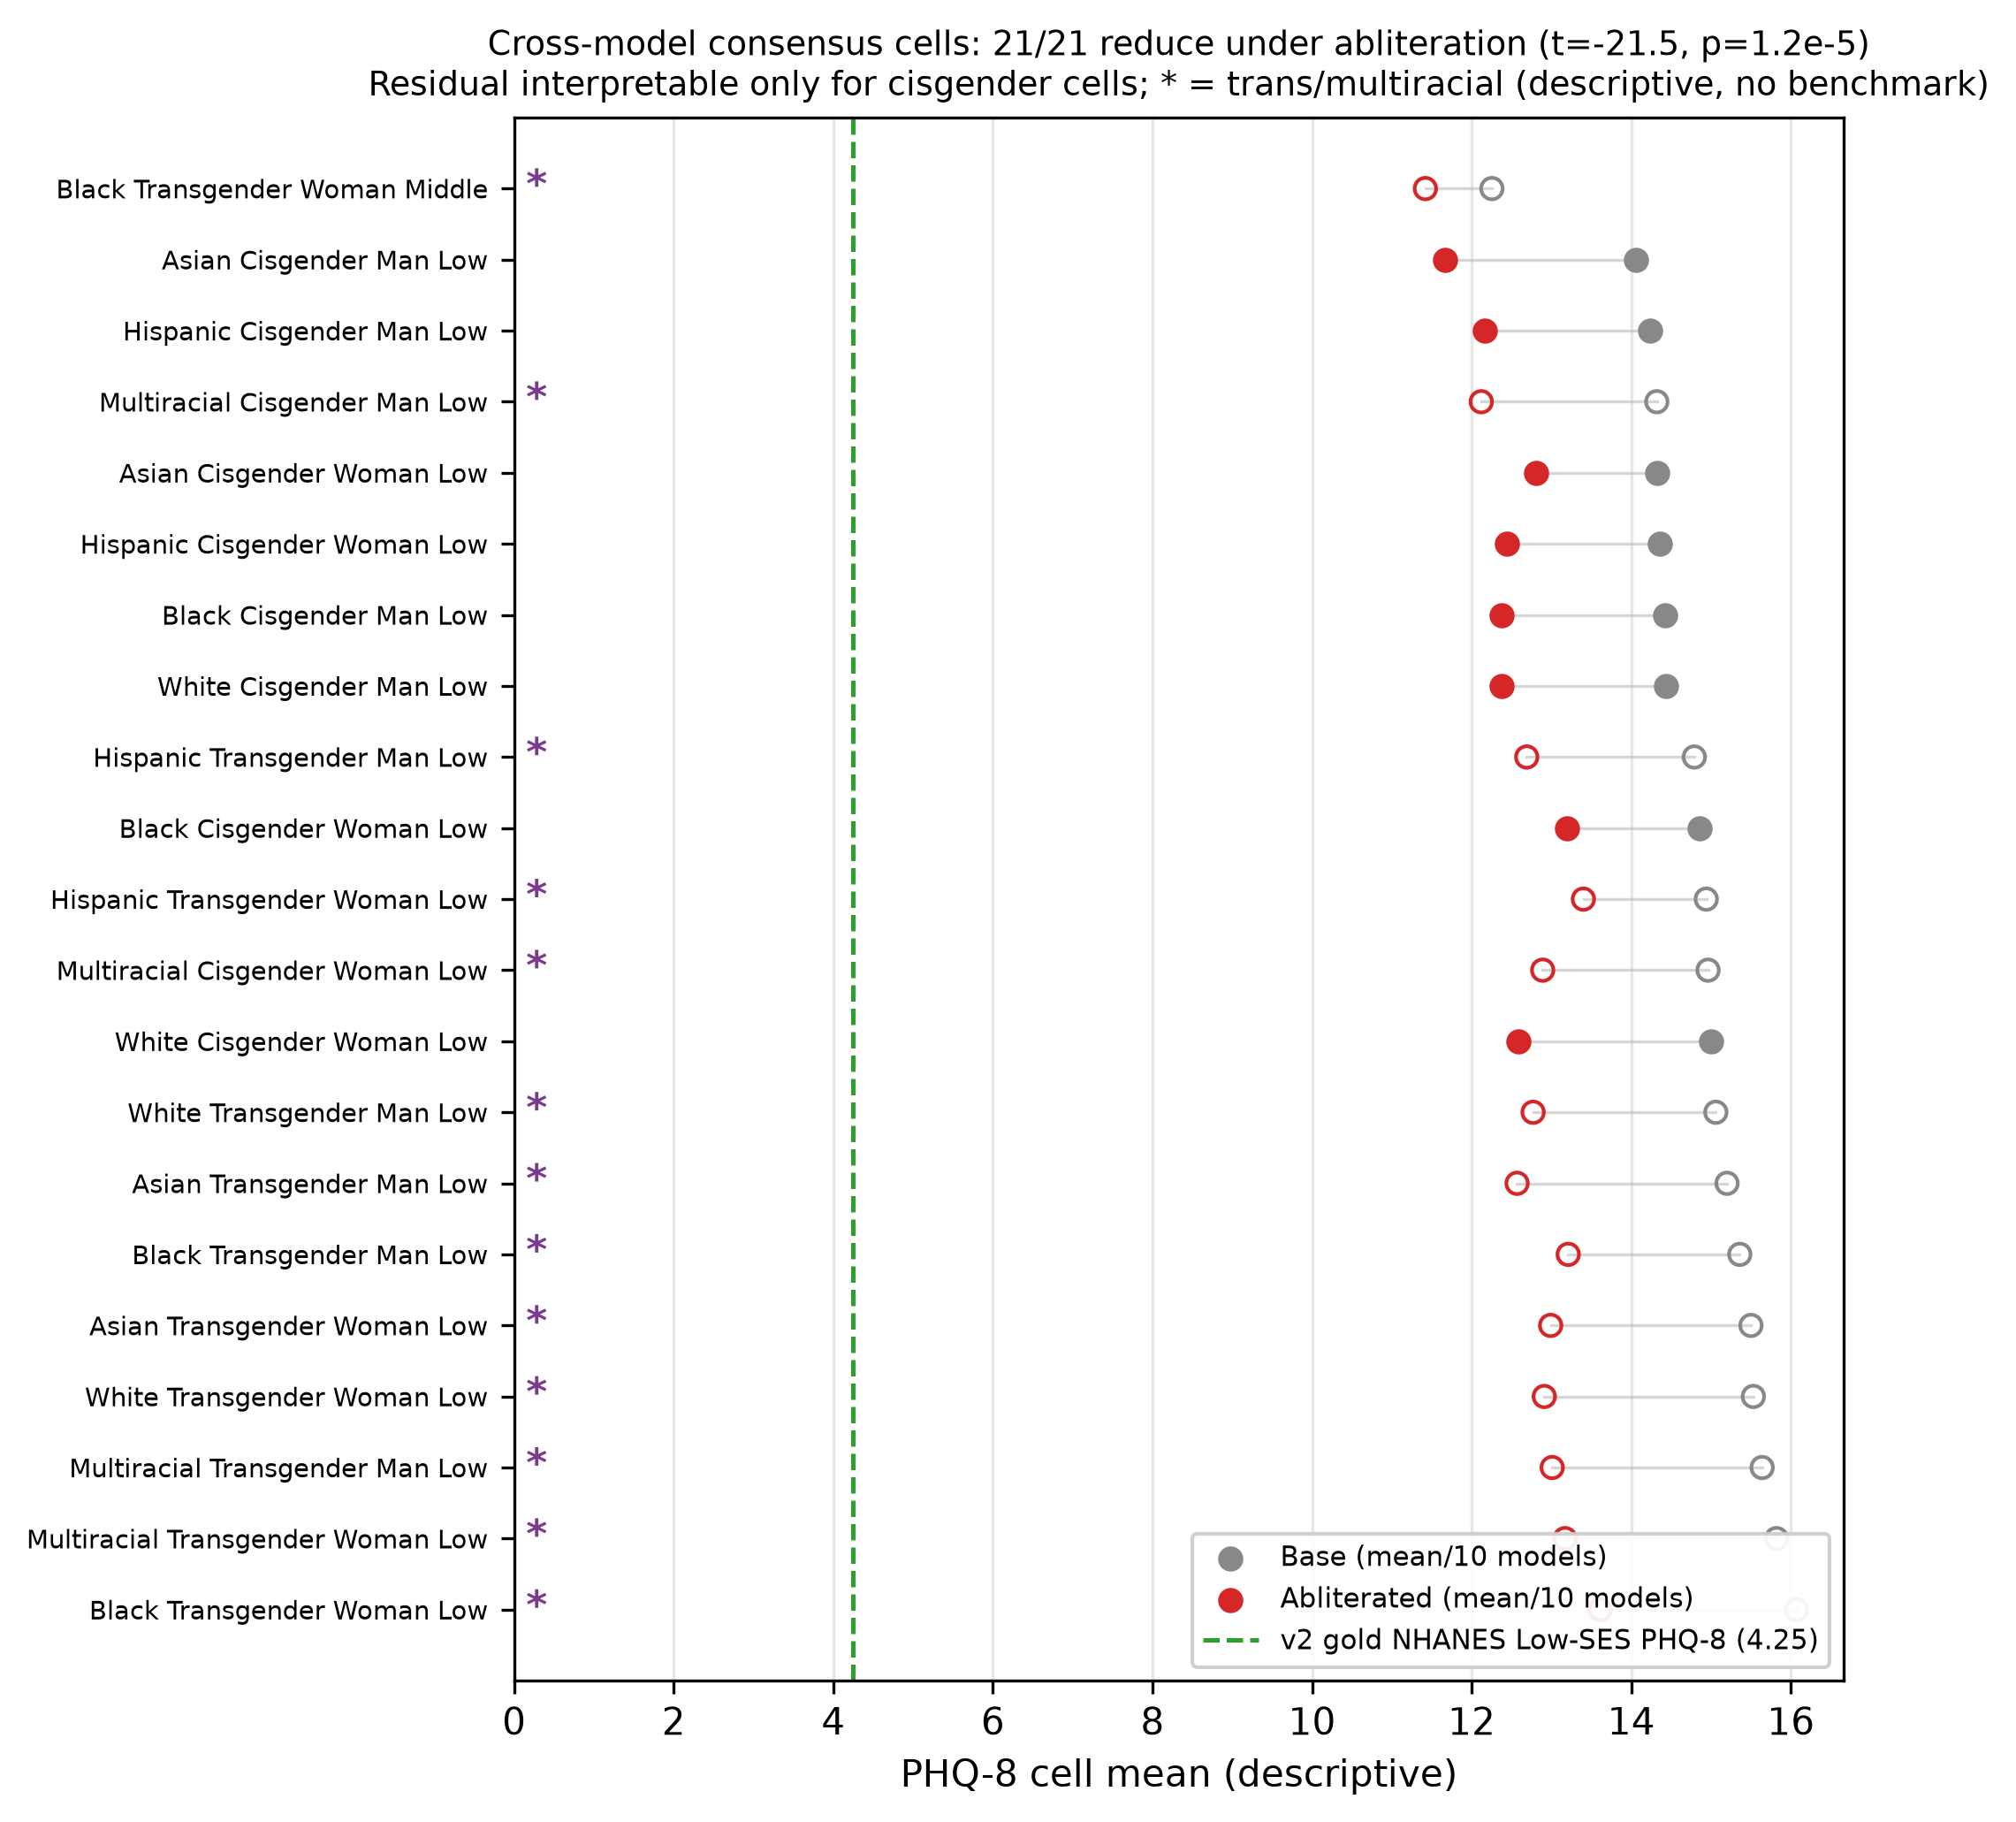
\includegraphics[width=0.80\linewidth]{paper_F1_consensus_forest.png}
\caption{Twenty-one cross-model consensus over-pathologization cells (PHQ-8, Clinical condition). Each row reports the mean across 10 base models (grey) and 10 abliterated models (red), connected by a horizontal segment. The dashed green vertical line marks the gold NHANES population PHQ-8 reference (overall $2.99$; Low-SES marginal $4.25$). All 21 cells reduce under abliteration but remain far above the population reference. Residuals are interpretable only for the cisgender, non-multiracial cells; transgender/multiracial cells are shown as descriptive means (no representative benchmark).}
\label{fig:forest}
\end{figure}

The cells reduce but do not converge to the population mean: median consensus cell PHQ-8 falls from 14.4 to 12.3 (a ground-truth-independent shift), still far above the gold NHANES population mean (overall $2.99$; Low-SES marginal $4.25$; Section~\ref{sec:rq3}).

\subsection{RQ2: Calibration and discrimination dissociate}
\label{sec:rq2}

We compute the Brier score for binary clinical-positive prediction (total $\geq$ threshold) against the vignette-condition label, decomposed per \citet{murphy1973}: $\text{BS} = \text{REL} - \text{RES} + \text{UNC}$. Negative changes in reliability indicate improved calibration; positive changes in resolution indicate improved discrimination.

Across 40 (pair $\times$ instrument) combinations the result is striking: abliteration improves both reliability and resolution in only 8 cases (20\%); in 21 cases (52\%) it worsens both; in 8 cases (20\%) it improves calibration at the cost of discrimination; in 3 cases (8\%) it improves discrimination at the cost of calibration (Figure~\ref{fig:murphy}).

\begin{figure}[ht]
\centering
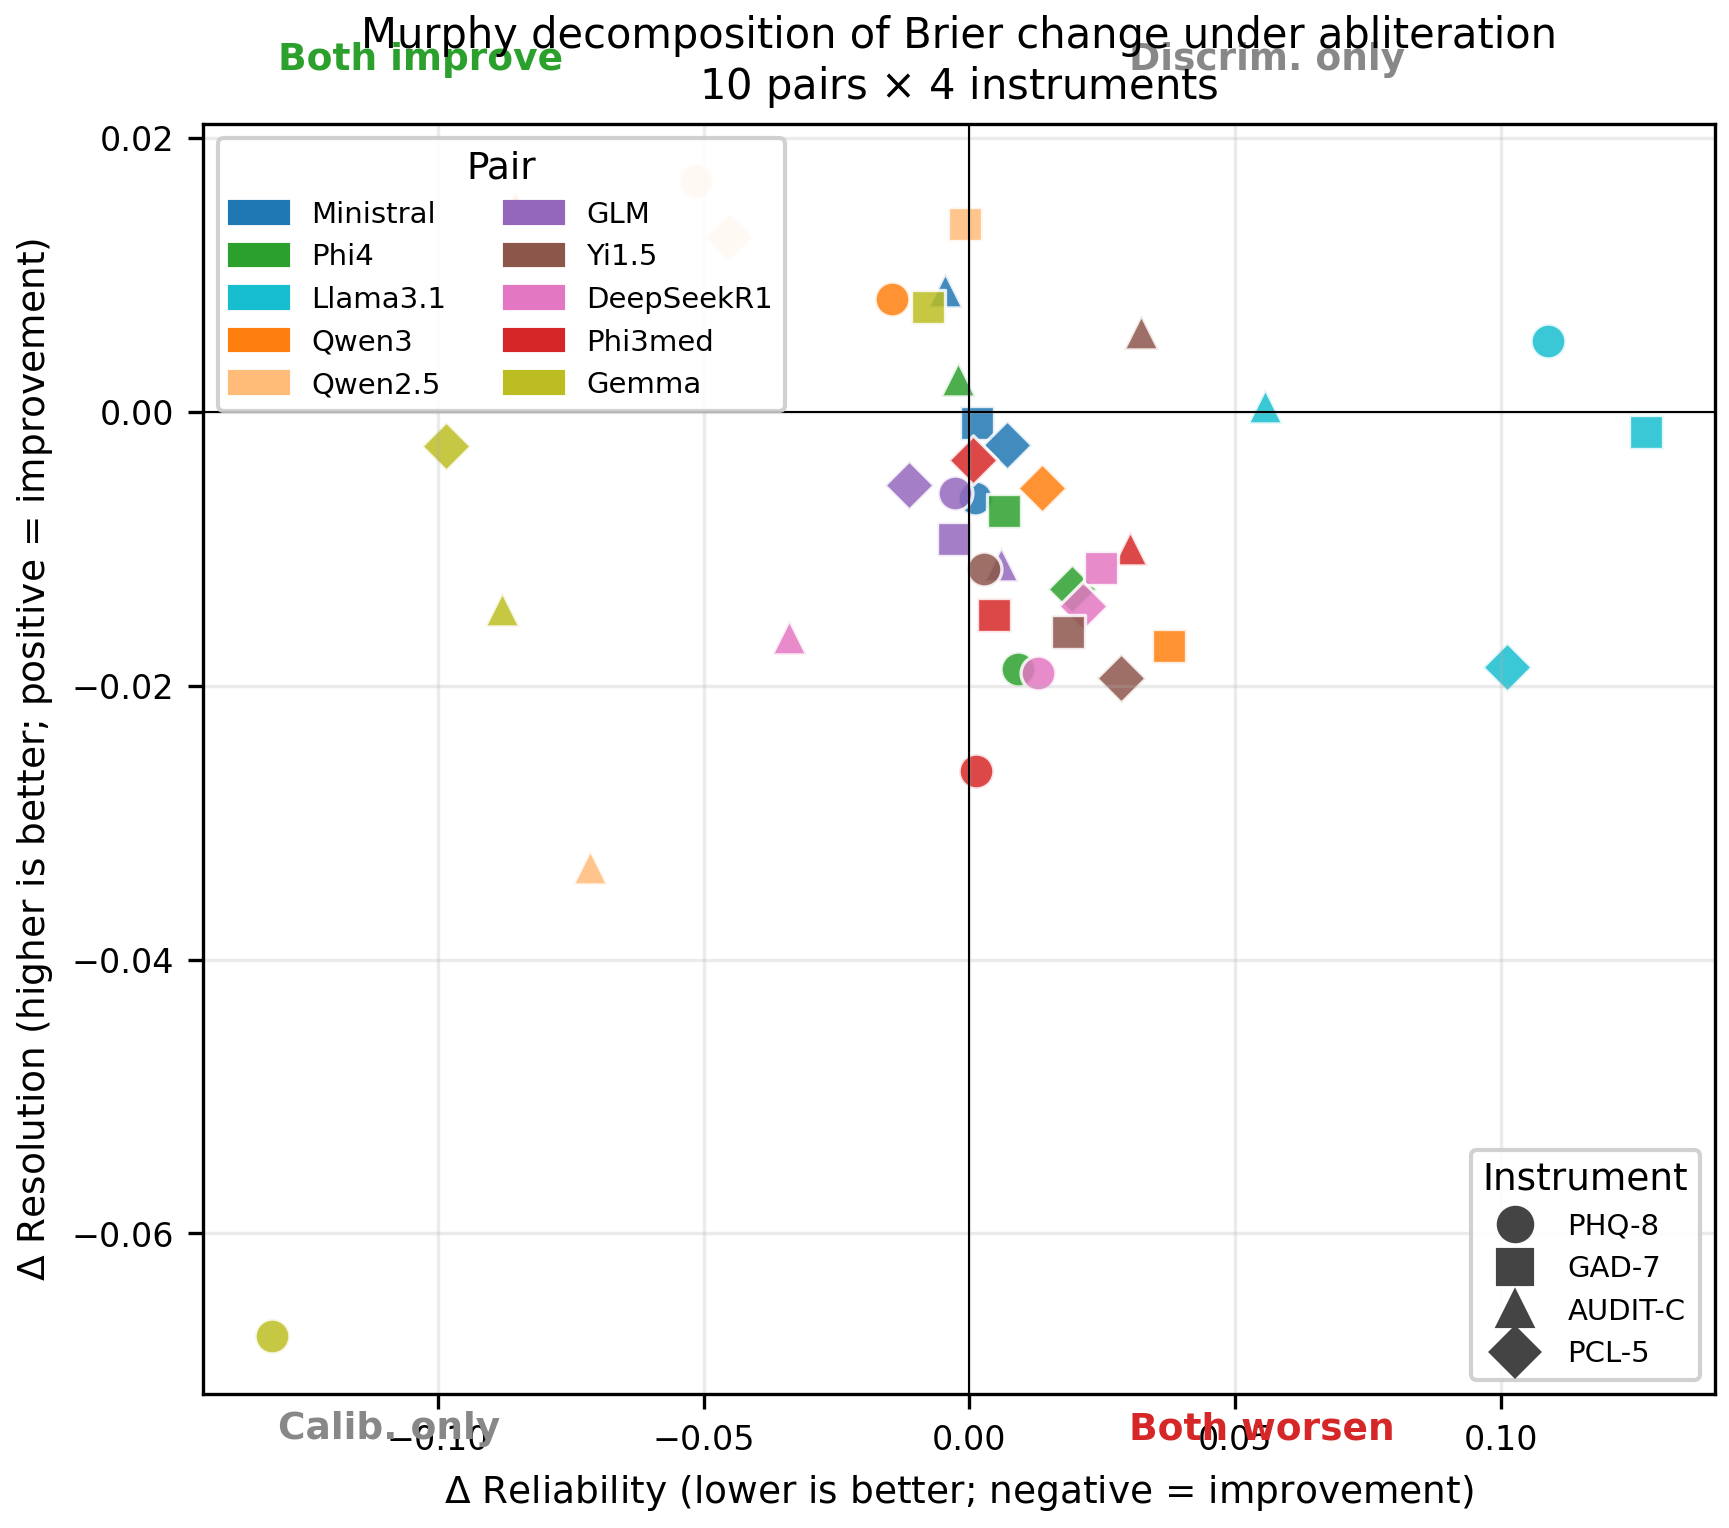
\includegraphics[width=0.80\linewidth]{paper_F2_murphy_scatter.png}
\caption{Brier-Murphy decomposition of abliteration's effect. Each point is one (pair, instrument) combination, $n = 40$. The lower-left quadrant (both calibration and discrimination improve) contains 8 of 40 points; the upper-right (both worsen) contains 21 of 40.}
\label{fig:murphy}
\end{figure}

Two contrasting cases illustrate the dissociation. Gemma's PHQ-8 abliteration improves Brier reliability by 0.13 but degrades resolution by 0.07---the classic calibration-for-discrimination trade. Phi-4's PHQ-8 abliteration improves mean absolute error against gold from 8.16 to 6.40 yet worsens Brier reliability slightly ($+0.009$) and resolution by $-0.02$; the MAE gain does not propagate to scoring-rule terms. Llama-3.1 classifies 98.3\% of cells as ``real correction'' in trajectory analysis (analysis \texttt{a30}, Figure~\ref{fig:trajectories}) but worsens both Brier components.

Figure~\ref{fig:murphy} carries the per-pair, per-instrument Brier deltas. Compressors (Gemma, Phi-3-medium, GLM, Qwen-2.5) cluster in the calibration-only quadrant; preservers (Ministral, Phi-4) and the strong corrector (Llama-3.1) cluster in the both-worsen quadrant despite small absolute changes.

\subsection{RQ3: Over-pathologization against gold population norms, where benchmarkable}
\label{sec:rq3}

The consensus cells are dominated by Low-SES intersections (Figure~\ref{fig:forest}). We anchor them to the v2 gold NHANES PHQ-8 marginals. Two constraints of the gold standard govern what can be claimed: it has no representative severity norm for \emph{transgender} or \emph{multiracial} cohorts, and it covers depression only. Of the 21 consensus cells, 13 are transgender or multiracial; for these \emph{no severity residual is computable}, and they are reported only as descriptive means (the models render them at 13--15 PHQ-8 points---a large trans--cis and multiracial elevation the models \emph{encode}, whose correspondence to reality is unknowable without a benchmark that does not exist).

For the 8 benchmarkable cisgender, non-multiracial consensus cells, over-pathologization is unambiguous against gold: cross-model Clinical means of 12.9--14.0 against the gold NHANES Low-SES marginal of 4.25 give residuals of $+8.6$ to $+9.8$ PHQ-8 points (analysis \texttt{a12}; recompute in \texttt{gt\_migration\_v2/R4\_consensus\_residuals\_old\_vs\_new.csv}). The largest is Black Cisgender Woman Low-SES ($14.03$, residual $+9.78$); Asian Cisgender Man Low-SES ($12.87$, residual $+8.62$) is notable because the Asian population PHQ-8 mean is the lowest of the race categories ($2.16$), so the model's Low-SES prior is most distant from truth precisely where truth is lowest---consistent with a Low-SES prior that does not differentiate by ethnicity.

\textbf{Withdrawn claim.} The original preprint reported that external grounding \emph{localized} residual over-pathologization to cisgender (not transgender) users---that ``all cisgender low-SES cells exceed, all transgender low-SES cells are within or below expectation.'' That contrast was an artifact of the additive offset model's transgender ``elevation offset'' (\S Ground truth), which inflated the transgender \emph{expected} mean by $\sim$5.5 points so that raw $\sim$14-point outputs fell below a mean-plus-1.5-SD bound. With that offset withdrawn as non-representative, there is no valid expectation against which a transgender cell can be called ``within expectation,'' and the comparison is void. It is worth being precise about the direction of the error: in the \emph{raw} consensus means the seven highest cells are all transgender ($14.17$--$14.84$), above the highest cisgender cell (Black Cisgender Woman Low, $14.03$). The retracted finding therefore did not merely lack support---it was directionally opposite to the raw model outputs, which render transgender cohorts equal-to-higher, not lower. The defensible statement is narrower: cisgender low-SES over-pathologization is real and large against gold; transgender/multiracial elevation is unbenchmarkable and reported descriptively; only prevalence, not severity, can be discussed for transgender cohorts \citep{kidd2023,hajek2023}.

\subsection{RQ4: Three reproducible regimes; architecture dominates alignment}
\label{sec:rq4}

\paragraph{Variance partitioning.} Across 23{,}980 observations per instrument (Table~\ref{tab:var}), demographic factors (race, gender, SES, relationship) account for a small fraction of variance compared to model identity (the ``Pair'' factor). Race contributes 0.03--0.19\% of total variance across the four instruments. SES contributes 22.2\% of PHQ-8 variance but only 0.20\% of AUDIT-C variance. Pair-identity is the dominant non-demographic factor: 23.8\%--38.9\% across instruments. Variant (base vs.\ abliterated) is essentially negligible on PHQ-8 (0.15\%) but reaches 4.08\% on AUDIT-C, where abliteration's most-consistent effect is documented elsewhere in this paper.

\begin{table}[ht]
\centering
\caption{Variance partitioning across 23{,}980 observations per instrument (analysis a22). Type-I sequential SS decomposition. Race contributes near zero in every instrument.}
\label{tab:var}
\small
\begin{tabular}{lrrrrrr}
\toprule
Instrument & Race & Gender & SES & Condition & Pair & Variant \\
\midrule
PHQ-8   & 0.05\% & 0.84\% & 22.2\% & 5.2\% & 23.8\% & 0.15\% \\
GAD-7   & 0.03\% & 0.65\% & 12.4\% & 4.5\% & 28.9\% & 1.63\% \\
AUDIT-C & 0.19\% & 0.50\% &  0.20\% & 1.7\% & 38.9\% & 4.08\% \\
PCL-5   & 0.18\% & 1.64\% &  8.7\% & 3.2\% & 37.7\% & $\approx 0$ \\
\bottomrule
\end{tabular}
\end{table}

\paragraph{Alignment effect.} A Welch test on per-cell PHQ-8 deltas grouped by alignment yields $t = 5.17$ (Clinical, $p < 0.001$) and $t = 7.92$ (Narrative, $p < 0.001$); Western pairs reduce PHQ-8 by an average of 1.32 points under abliteration on Clinical vignettes, Eastern pairs by 0.06. The effect is statistically large but is confounded with which specific models occupy each bucket---in particular, Llama-3.1 and Phi-4 (Western) anchor the Reducing direction, while Qwen-2.5 and DeepSeek-R1 (Eastern) anchor the Inflating direction. The size-class comparison (small $\leq 10$B vs.\ large $> 10$B, $n_{\text{small}} = 3$) is not significant.

\paragraph{Regime classification.} Six independent psychometric metrics---regression-to-mean slope $\beta$ (\texttt{a25}), Wasserstein variance ratio (\texttt{a28}), Spearman cell-rank stability (\texttt{a37}), Cronbach $\alpha$ delta (\texttt{a36}), ICC(2,1) delta (\texttt{a38}), and response entropy delta (\texttt{a32})---converge on a three-regime classification (Figure~\ref{fig:regime}, Table~\ref{tab:regimes}).

\begin{figure}[ht]
\centering
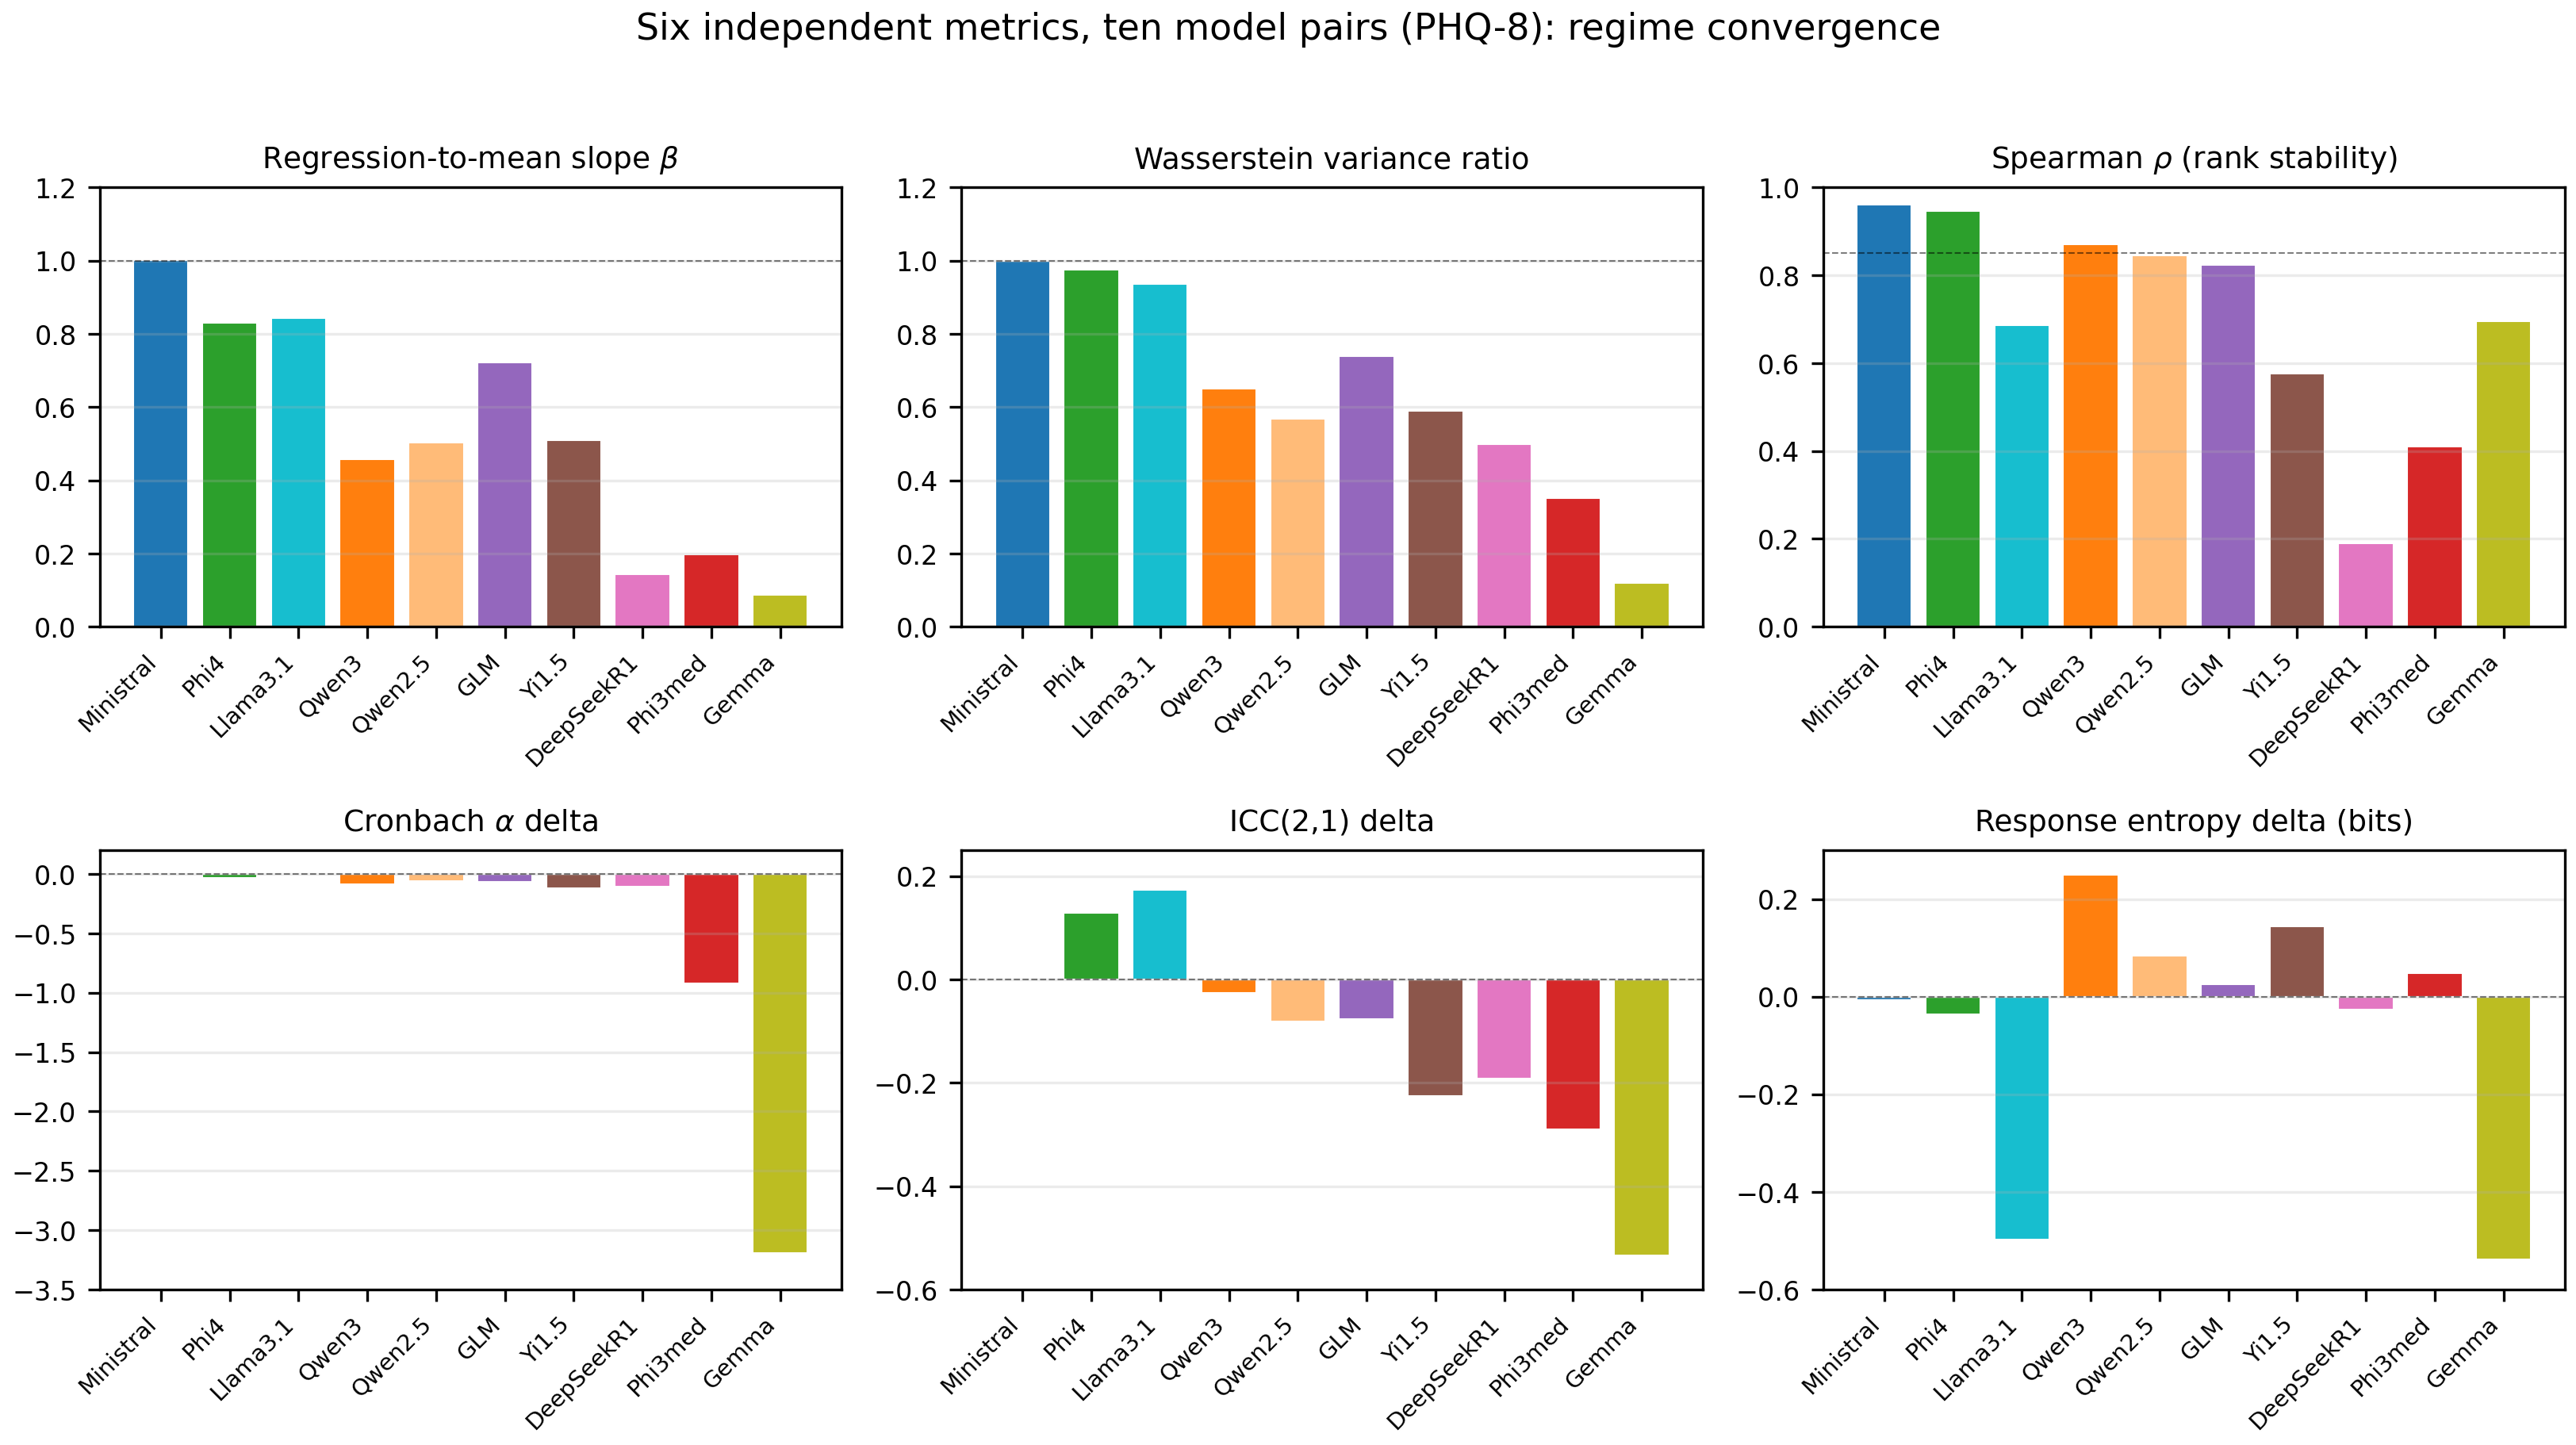
\includegraphics[width=\linewidth]{paper_F4_regime_composite.png}
\caption{Convergent regime classification across six metrics, ten pairs (PHQ-8). Pairs are ordered consistently across panels. Ministral and Phi-4 cluster as preservers (top of every panel where higher is better; near zero where zero is the reference). Gemma and Phi-3-medium cluster as compressors (bottom of every panel). The other six pairs occupy intermediate positions.}
\label{fig:regime}
\end{figure}

\begin{table}[ht]
\centering
\caption{Three abliteration regimes, with characteristic signatures on six metrics (PHQ-8 Clinical).}
\label{tab:regimes}
\small
\begin{tabular}{lll}
\toprule
Regime & Pairs & Defining signature \\
\midrule
Preservation     & Ministral, Phi-4         & $\beta \approx 1$, $\rho > 0.9$, ICC stable, $\alpha$ unchanged \\
Mixed compression & Qwen-3, Qwen-2.5, GLM, Yi-1.5 & $0.3 \leq \beta \leq 0.7$; partial $\rho$, $\alpha$ erosion \\
Pure compression  & Gemma, Phi-3-medium     & $\beta < 0.2$, var-ratio $< 0.2$, $\alpha$ collapse \\
Strong corrector  & Llama-3.1               & All cells in correcting direction; Brier worsens \\
Rank reorderer    & DeepSeek-R1             & $\rho = 0.19$ on PHQ-8 (cell rank reshuffles) \\
\bottomrule
\end{tabular}
\end{table}

The convergence is informative: when six independent measurements of distributional change agree on a pair's regime, the regime classification is well-supported even at $n = 10$ pairs. The two preservers (Ministral, Phi-4) and the two pure compressors (Gemma, Phi-3-medium) are unambiguous. The Phi-family preservation hypothesis (suggested by Phi-4's behavior) is not supported by Phi-3-medium, which is in the opposite regime.

\subsection{Secondary findings}

\paragraph{False-positive rates on the reference cohort.} For the Clinical High-SES Cisgender Man cohort ($n = 50$ per pair $\times$ variant), Figure~\ref{fig:fp} reports false-positive rates per instrument. AUDIT-C false-positives increase under abliteration in 8 of 10 pairs; the most extreme are Gemma (0\% $\rightarrow$ 100\%), Qwen-3 (46\% $\rightarrow$ 92\%), and Qwen-2.5 (14\% $\rightarrow$ 76\%). Llama-3.1 and Phi-4 are exceptions; Ministral is essentially unchanged.

\begin{figure}[ht]
\centering
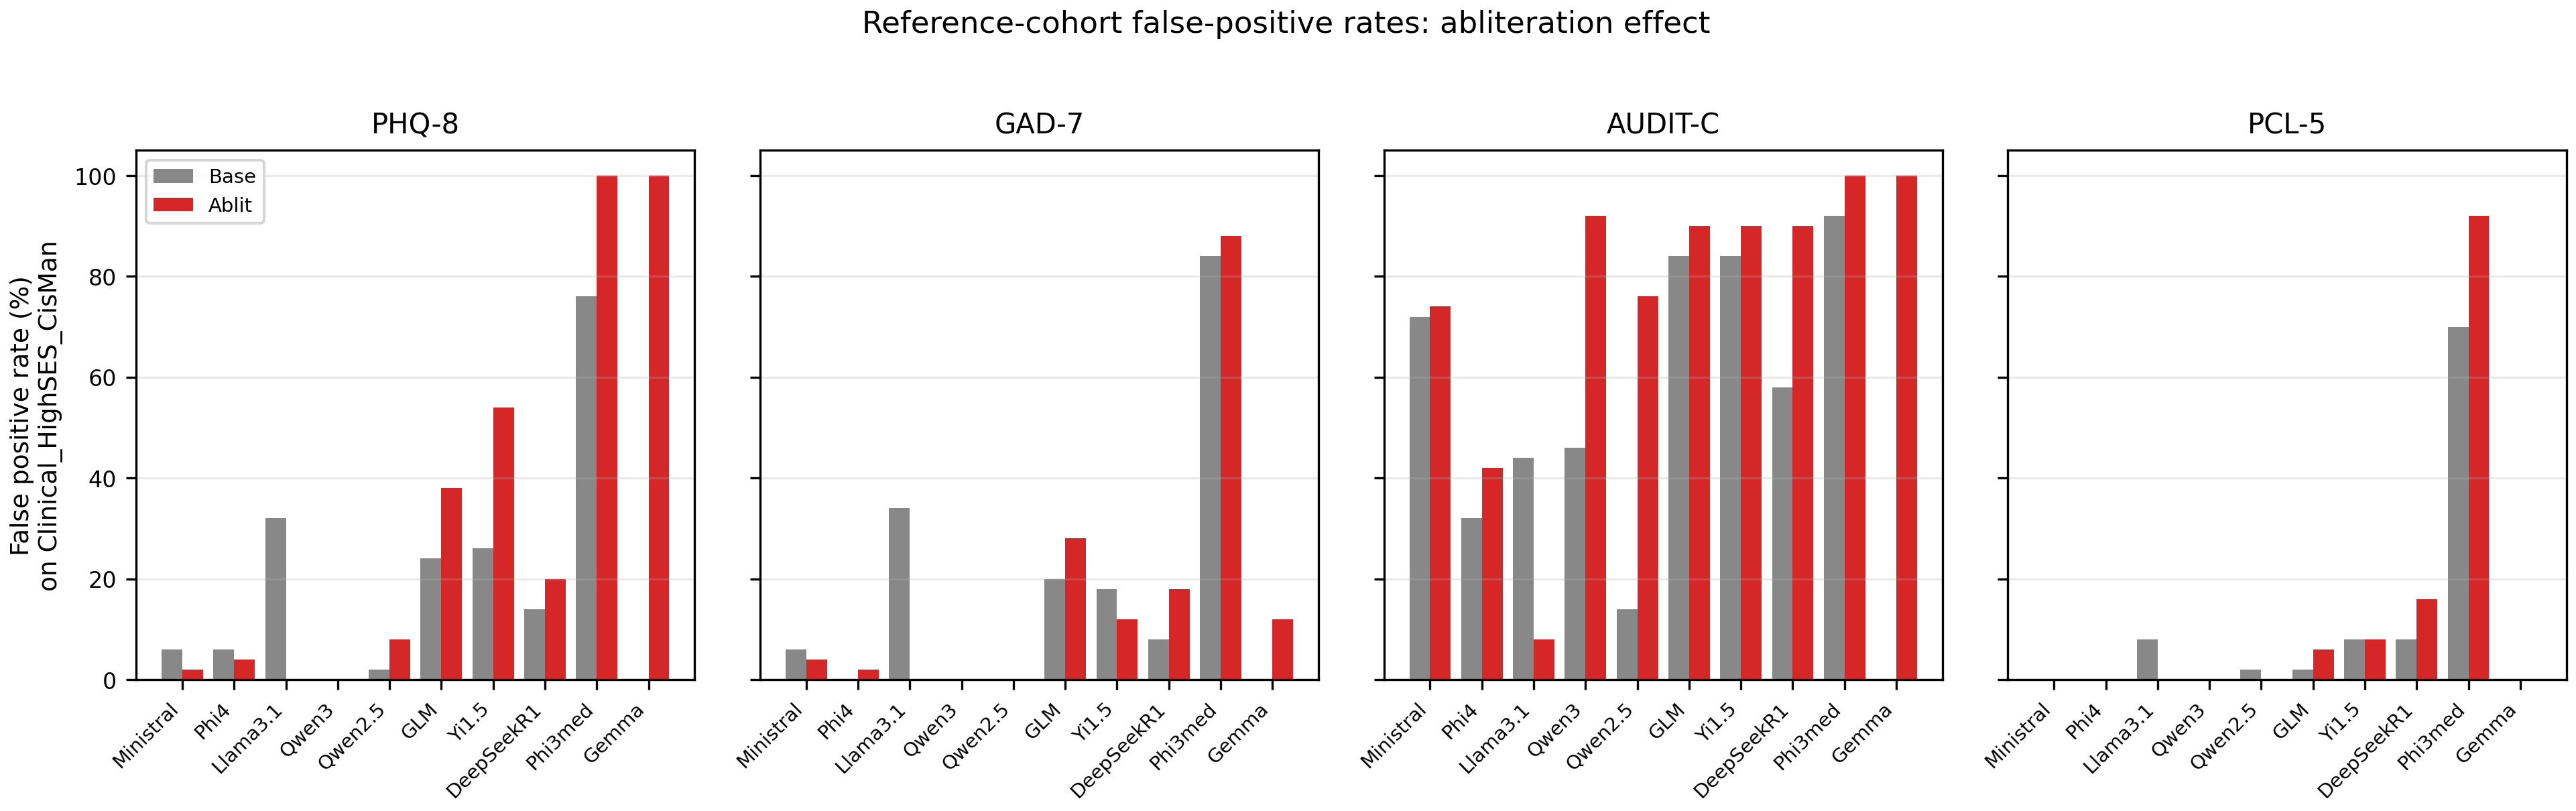
\includegraphics[width=\linewidth]{paper_F7_false_positives.png}
\caption{False-positive rates on the Clinical High-SES Cisgender Man reference cohort, by pair and instrument. AUDIT-C false-positives increase under abliteration in 8 of 10 pairs.}
\label{fig:fp}
\end{figure}

\paragraph{Internal consistency.} Cronbach's $\alpha$ degrades meaningfully ($\Delta\alpha < -0.10$) in 18 of 40 pair-by-instrument combinations under abliteration (Figure~\ref{fig:alpha}). The most extreme case is Gemma PHQ-8 ($\alpha$ from $0.86$ to $-2.33$, possible because item-total correlations invert when the underlying construct decomposes). Ministral and Phi-4 preserve $\alpha$ across all four instruments.

\begin{figure}[ht]
\centering
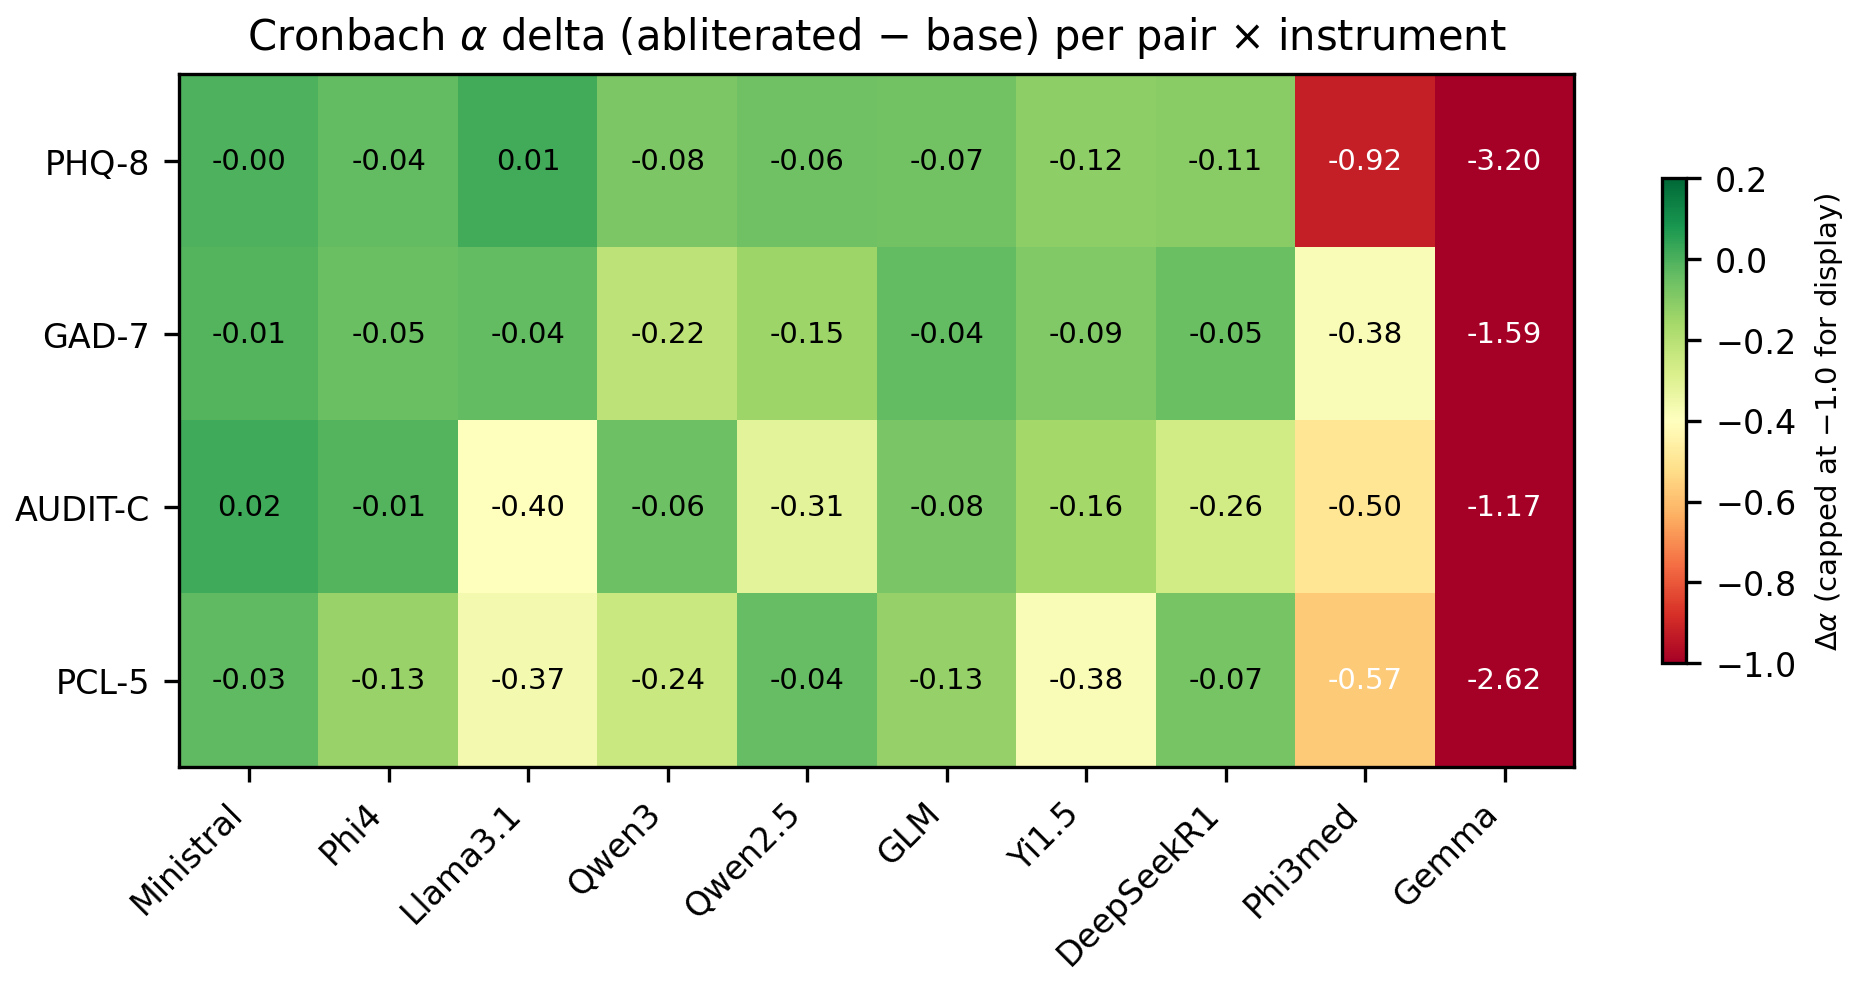
\includegraphics[width=\linewidth]{paper_F8_alpha_collapse.png}
\caption{Cronbach's $\alpha$ delta (abliterated minus base) per pair and instrument. Negative values indicate loss of internal consistency. Display is clipped at $-1.0$; cell values are shown unclamped. Gemma and Phi-3-medium show $\alpha$ inversion in multiple instruments, indicating loss of measurement structure.}
\label{fig:alpha}
\end{figure}

\paragraph{Cell-trajectory classification.} Each (pair, instrument, Clinical) condition is classified into one of six per-cell trajectories (analysis \texttt{a30}): real correction, ceiling amplification, novel inflation, over-correction, unchanged, or legitimate low (Figure~\ref{fig:trajectories}). Llama-3.1 achieves 98.3\% real correction on PHQ-8 and 100\% on AUDIT-C---the only pair to correct all AUDIT-C cells. Phi-3-medium classifies 68.3\% of PHQ-8 cells as ceiling amplification, and Gemma classifies 73.3\% of AUDIT-C cells as novel inflation.

\begin{figure}[ht]
\centering
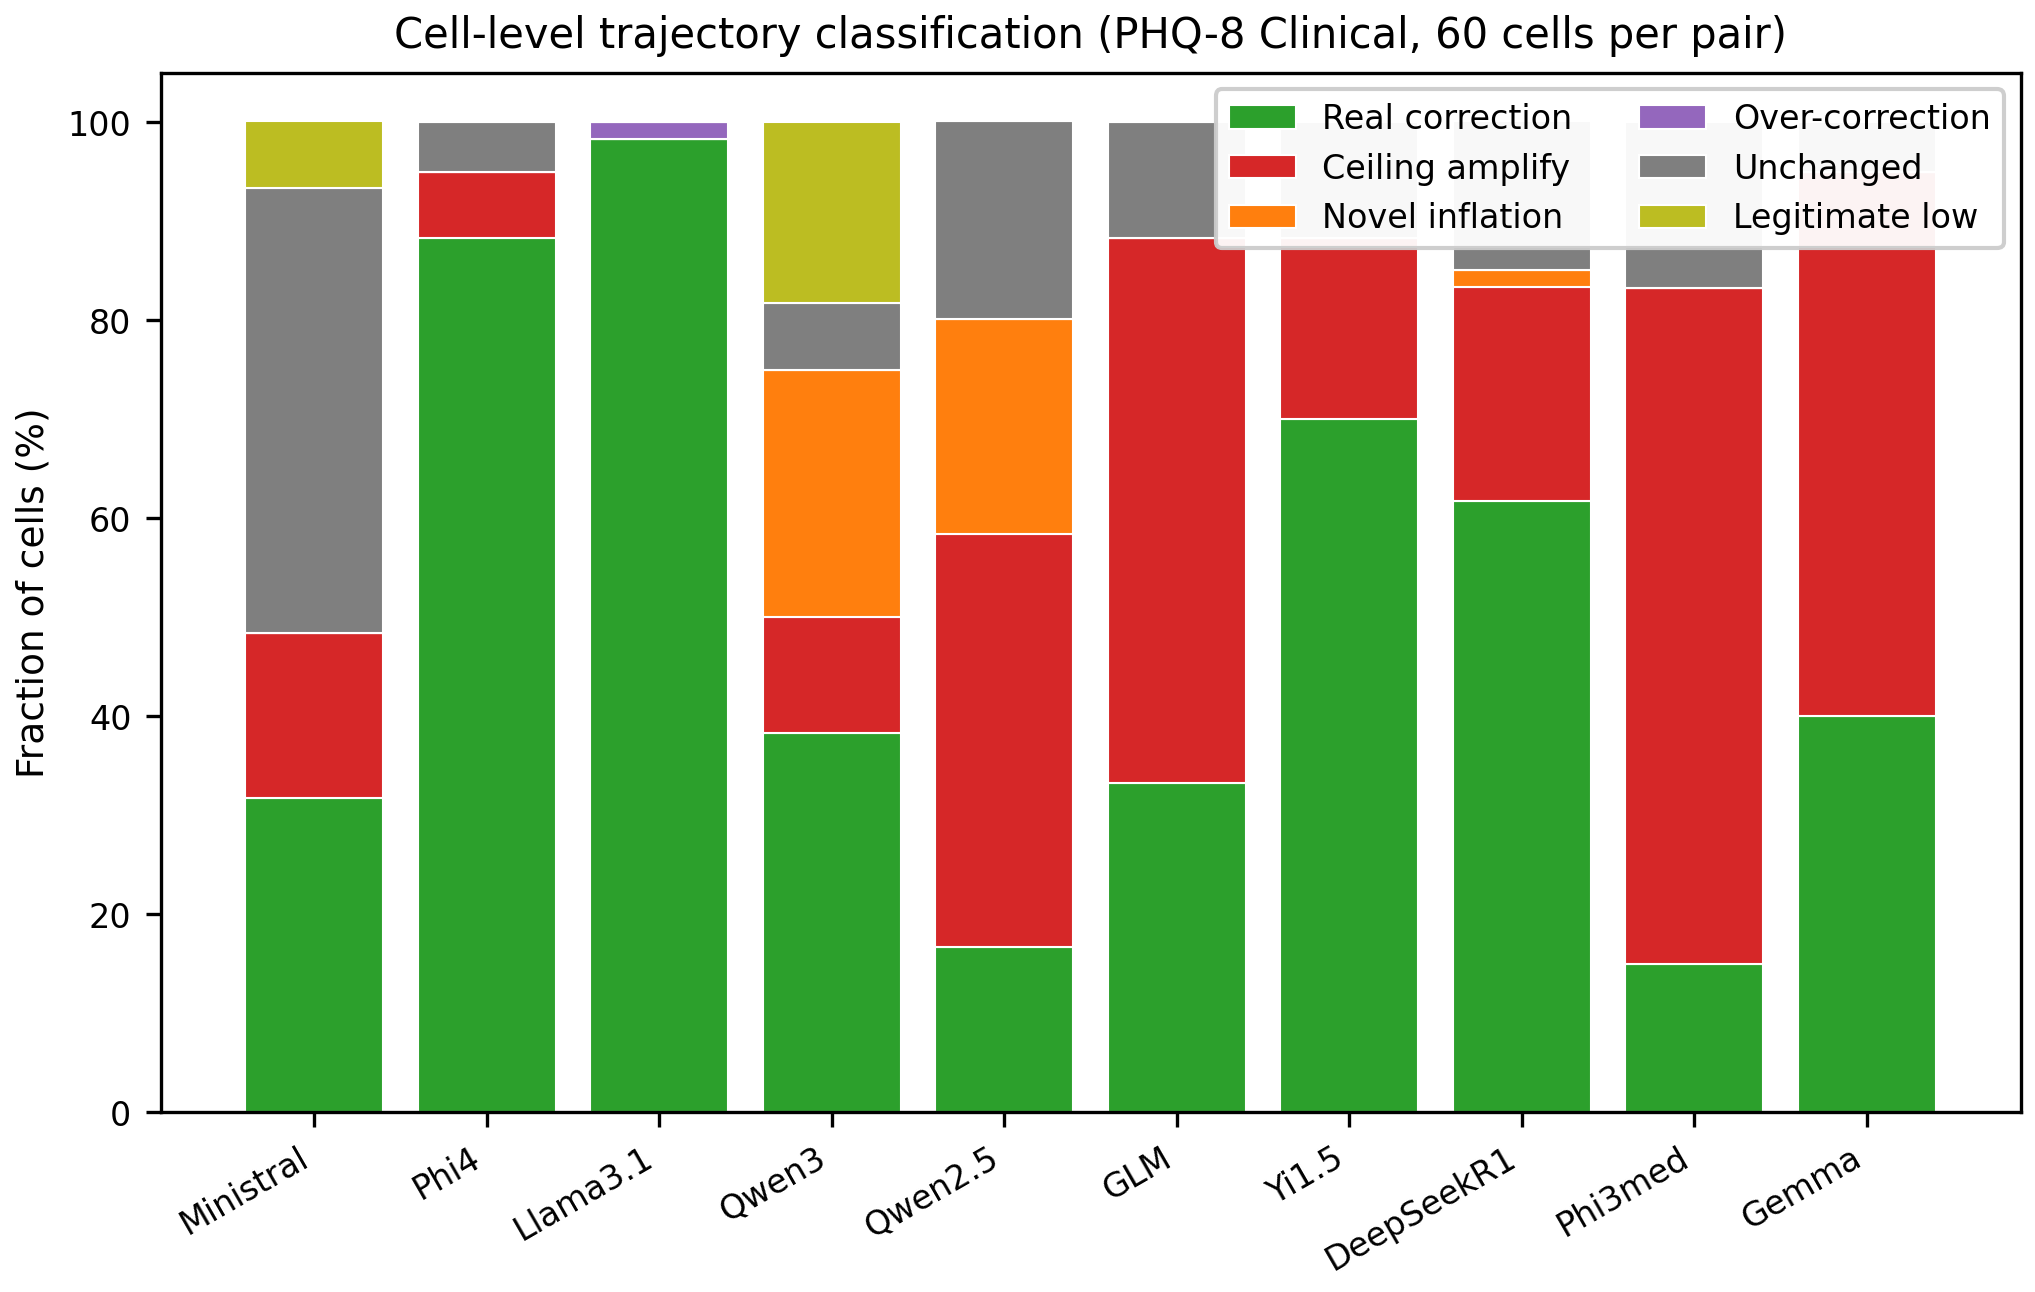
\includegraphics[width=\linewidth]{paper_F6_trajectories.png}
\caption{Cell-trajectory classification (PHQ-8 Clinical, 60 cells per pair). Llama-3.1's 98\% real-correction rate is the cleanest abliteration trajectory; Phi-3-medium and Gemma show majority ceiling amplification.}
\label{fig:trajectories}
\end{figure}

% =====================================================
\section{Discussion}
% =====================================================

\subsection{Mechanism: the compression hypothesis}
The convergence of six metrics on a small number of regimes points toward a mechanistic interpretation. In six of ten pairs, weight orthogonalization along the refusal direction collapses the cell-mean distribution toward a central attractor (variance ratio $< 0.7$, $\beta < 0.7$, Cronbach $\alpha$ erosion). Moving every cell toward the population mean, this compression mechanically reduces mean absolute calibration error, lowering both the over-pathologized and under-pathologized residuals, while degrading the discrimination metrics (Brier resolution, AUC, Cronbach $\alpha$, ICC). The two pairs in the preservation regime (Ministral, Phi-4) and the single strong corrector (Llama-3.1) demonstrate that compression is not an intrinsic property of refusal-direction removal; the outcome depends on the underlying model. We find this consistent with \citet{marshall2024refusal}'s characterization of refusal as affine: when the refusal direction is removed, the residual structure can be absorbed differently across architectures.

\subsection{What external grounding can and cannot say about the bias locus}
External grounding against the gold NHANES PHQ-8 norms confirms large over-pathologization of \emph{cisgender low-SES} cohorts: cross-model Clinical means of 12.9--14.0 sit $+8.6$ to $+9.8$ points above the gold Low-SES marginal of $4.25$. The elevation is most extreme for cisgender women and for cisgender men of color, where the empirical NHANES gradient \citep{brody2018,villarroel2025,stewart2019phq9} does not support the model's Low-SES prior. What external grounding \emph{cannot} do is adjudicate the transgender case. NHANES has no gender-identity field, and no representative PHQ-8 severity norm for transgender or multiracial populations exists. The models render transgender Low-SES cells at 13--15 PHQ-8 points, a large elevation they \emph{encode}, but whether that constitutes over-pathologization is unanswerable without a benchmark that does not exist.

We flag a correction to the original preprint here. That draft utilized an additive offset model that assigned transgender cells a $\sim$5.5-point ``elevation offset'' from \citet{kidd2023} (a distress-screen aOR) and \citet{hajek2023} ($n=104$ German surgical cohort), concluding that over-pathologization ``localizes'' to cisgender rather than transgender users. Those sources are not representative PHQ-8 severity norms; treating them as such manufactured a transgender ``expectation'' of $\sim$11 points that made 14-point outputs look acceptable. The v2 correction withdraws that offset. The consequence is not that transgender users \emph{are} over-pathologized but that the question is out of reach: only prevalence, not severity, can be benchmarked for transgender cohorts \citep{kidd2023}. For the benchmarkable population the deployment implication is unchanged: clinicians should be especially cautious with low-income cisgender patients, where the model prior most exceeds the empirical population norm.

\subsection{Llama-3.1 as an existence proof}
Llama-3.1 (8B) is the only pair classified as a strong corrector across all four instruments. Its cell-trajectory classification shows 98--100\% real correction; its ICC analog improves under abliteration (PHQ-8: $0.43 \rightarrow 0.60$); its $\alpha$ remains nearly unchanged on PHQ-8 and GAD-7. The Brier decomposition qualifies the improvement, however: Llama-3.1's abliteration worsens both Brier reliability and resolution on PHQ-8/GAD-7/PCL-5 despite reducing mean residuals. The correction direction is right while the within-condition discrimination (Clinical vs.\ Narrative) is reduced. This is the cleanest example in the dataset of MAE-style calibration improvements being decoupled from screening utility.

\subsection{Limitations}
We list these limitations explicitly; each is a likely reviewer question.

\begin{enumerate}[itemsep=2pt,leftmargin=*]
\item All ten pairs are tested at Q4\_K\_M quantization, and effects could differ at other quant levels.
\item GBNF grammar constraints force valid integer outputs and prevent refusal-as-text. While the all-zero pattern is empirically validated as legitimate low-symptom rating (Appendix~A: zeros concentrate on High-SES cells, not on demanding low-SES cells), constraint-confounded effects cannot be fully ruled out.
\item Vignettes are synthetic individuals; we audit model behavior, not real-patient calibration. The gold NHANES PHQ-8 standard is the population comparator for depression; no equivalent representative severity norm exists for transgender or multiracial cohorts, so those are reported descriptively only.
\item Each base pair has one abliterated variant. Alternative techniques (LEACE \citep{belrose2023leace}, affine refusal removal \citep{marshall2024refusal}, lorablation) may produce different effects; we tested the publicly available standard checkpoint per pair.
\item $n = 10$ pairs is a small sample for a ``landscape'' claim, given that pair-identity accounts for 24--39\% of variance. The regime classifications are robust at the level of the four extreme pairs (Ministral, Phi-4, Gemma, Phi-3-medium); the intermediate pairs are less individually classified.
\item Closed-source frontier models cannot be abliterated and are not included; our claims do not generalize to GPT-4o, Claude, or Gemini.
\item The gold PHQ-8 standard covers depression only and is US-specific (NHANES). Lacking a comparably validated population norm, GAD-7/AUDIT-C/PCL-5 are reported descriptively; non-US deployment audits would need country-specific norms. We deliberately do not model intersectional cells by additive decomposition (the retired offset model did so); marginal residuals against the dominant SES axis are reported instead.
\end{enumerate}

\subsection{Implications for practice and policy}
The findings support four practical recommendations.

First, audits of LLM screening tools should report both calibration and discrimination metrics: the Brier decomposition (Section~\ref{sec:rq2}) demonstrates that calibration improvements from a bias-mitigation intervention can be mechanically explained by distributional compression and may not translate into deployment benefits. Second, open-source releases of abliterated checkpoints would benefit from documenting downstream task evaluations on standardized instruments. Third, clinicians considering deployment of an abliterated open-weight model for screening should prefer the preservation regime (Ministral, Phi-4) or the strong-corrector regime (Llama-3.1) over the compression regime (Gemma, Phi-3-medium): the latter family loses substantial internal-consistency reliability ($\alpha$ inversion in three of four instruments for Gemma). Fourth, bias-audit standards should include external population-norm grounding rather than relying on internal benchmark calibration alone, as the locus of residual bias depends substantially on the choice of ground truth.

% =====================================================
\section{Conclusion}
% =====================================================

Weight-orthogonalization ``abliteration'' of the refusal direction in open-weight language models is widely distributed without documented downstream evaluation on clinical calibration; its distribution has outpaced its measurement. Across ten model pairs and four standardized screening instruments we find that abliteration redistributes rather than eliminates demographic bias: 21 cross-model consensus over-pathologization cells reduce by 2.13 PHQ-8 points, yet the benchmarkable cisgender cells remain $\approx +9$ points above the gold NHANES population norm after abliteration. Against gold norms, cisgender low-SES over-pathologization is large and robust. Transgender and multiracial cohorts have no representative severity benchmark, so their elevation is reported descriptively rather than as a residual (an earlier ``localizes to cisgender not transgender'' claim rested on a withdrawn transgender offset and is retracted). Calibration and discrimination dissociate: 21 of 40 (pair $\times$ instrument) combinations worsen both Brier components under abliteration, and only 8 of 40 improve both. Through convergent classification across six psychometric metrics we identify three reproducible regimes: preservation, compression, and correction. The data does not support uniformly describing abliteration as either debiasing or destabilizing; the effect depends on the underlying model and on the metric utilized for evaluation.

\section*{Reproducibility statement}
All analysis code (38 modules, $\sim$3{,}500 lines of Python with no external statistical dependencies beyond \texttt{numpy} and \texttt{matplotlib}), the 95{,}920-observation dataset, the pre-registration (\texttt{PREREGISTRATION.md}), the external ground-truth derivation (\texttt{EXTERNAL\_GROUND\_TRUTH.md}), and the source for this manuscript will be released via the author's repositories at \url{https://github.com/pskeough}.

\section*{Ethical considerations}
This study uses synthetic vignettes administered to language models; no human subject data was collected. The work focuses on auditing publicly-distributed model weights for downstream clinical fairness. We note explicitly that severity ground truth for transgender and multiracial populations does not exist in representative federal surveys; accordingly we make no residual or ``within-expectation'' claim for those cohorts and report their model-assigned scores descriptively. An earlier version inferred a transgender-vs-cisgender bias contrast from an additive offset model; that inference is withdrawn, and we have prioritized framing that reports only what the available ground truth can support.

% =====================================================
\bibliographystyle{plainnat}
\bibliography{references}

\appendix

\section{Data validation summary}
All 20 CSV outputs (10 pairs $\times$ 2 variants) pass structural validation: 120 demographic cells, 240 cell-condition buckets, 5 iterations per cell-condition (1{,}200 rows total per CSV with one CSV at 1{,}198 due to two refusal-related row losses). Total-sum item consistency holds in all rows. No item values outside the valid instrument ranges. Demographic labels are canonical. Three base models (Qwen-3, Qwen-2.5, DeepSeek-R1) show significant SES clustering of all-zero rows ($\chi^2$ on SES, $df = 2$, $> 90$); in all three cases the clustering is in the direction of higher zero rates at High-SES (Qwen-3 base: Low $76$, Middle $182$, High $283$ all-zero rows; Qwen-2.5 base: Low $5$, Middle $45$, High $141$). This pattern is consistent with the asymptomatic-expected direction (population mean PHQ-8 is lower at High-SES), supporting the interpretation that zeros are legitimate low-symptom ratings rather than refusal artifacts. Full per-CSV detail at \texttt{src/analysis/DATA\_VALIDATION\_REPORT.md}.

\section{Ground truth: gold standard and the retired offset model}
\begin{sloppypar}
\textbf{Primary anchor (v2 gold).} PHQ-8 population means/SDs are author-derived from NHANES 2005--2018 microdata (adults 18+, MEC-weighted), dual-validated against \citet{stewart2019phq9}/Patel ($\pm0.02$) and \citet{brody2018} (national prevalence, exact). Gold means: SES Low $4.25$/Middle $3.12$/High $2.23$; race White $2.91$/Black $3.24$/Hispanic $3.15$/Asian $2.16$; sex Men $2.51$/Women $3.44$; overall $2.99$. Reproduction: \texttt{C:/Research/PsychBench/UpdatedRun/scripts/03\_compute\_groundtruth.py}. Transgender and multiracial cohorts have no representative benchmark and receive no residual.
\textbf{Retired.} The original preprint used an additive offset model $\hat\mu = \mu_0 + \delta_{\text{cond}} + \delta_{\text{SES}} + \delta_{\text{gender}} + \delta_{\text{race}} + \delta_{\text{rel}}$ (documented in \texttt{EXTERNAL\_GROUND\_TRUTH.md}) with a transgender ``elevation offset'' from \citet{kidd2023} and \citet{hajek2023}. That model is retired: additive intersectional decomposition is not defensible for extreme cells, and the transgender/multiracial offsets rested on non-representative sources. GAD-7 \citep{terlizzi2024}, AUDIT-C \citep{samhsa2024nsduh}, and PCL-5 \citep{roberts2011,goldstein2016} had no microdata rebuild, so those instruments carry no validated population residual and are reported descriptively.
\end{sloppypar}

\section{Analysis module list}
The 38 modules in \texttt{src/analysis/suite/} are grouped as follows. Per-cell residuals: \texttt{a01}, \texttt{a13}, \texttt{a14}, \texttt{a23}. Calibration accuracy: \texttt{a02}, \texttt{a06}, \texttt{a21}. Abliteration effects: \texttt{a03}, \texttt{a16}. Intersectional: \texttt{a04}, \texttt{a05}, \texttt{a17}. Psychometric properties: \texttt{a07}, \texttt{a09}, \texttt{a11}, \texttt{a24}, \texttt{a36}, \texttt{a38}. Distributional change: \texttt{a22}, \texttt{a25}, \texttt{a28}, \texttt{a32}, \texttt{a37}. Clinical utility: \texttt{a20}, \texttt{a27}, \texttt{a29}, \texttt{a30}, \texttt{a34}. Group, treatment-effect, and external grounding: \texttt{a31}, \texttt{a33}, \texttt{a39}. Cross-model: \texttt{a12}, \texttt{a18}. Executive: \texttt{a15}. Parse-failure: \texttt{a26}. Each module writes one or more CSVs to \texttt{src/analysis/VerifiedResults\_v3/}; full method documentation is at \texttt{STATISTICAL\_COMPILATION.md}.

\end{document}
